\centerline{\bf \Huge Домашнее задание}
\centerline{\bf \Huge Антипараллельность+Степень точки.}

\begin{flushright}
        \scriptsize{Восьмиклассникам штрафов не будет(кроме Германа).}
\end{flushright}

\textbf{Определение.} \textit{Степенью точки} $X$ относительно окружности $\omega$ называется величина $\operatorname{Pow}(X, \omega)=d^2-R^2$, где $d-$ расстояние от точки $X$ до центра окружности, а $R$ - радиус окружности.

Если прямая, проходящая через точку $X$, пересекает $\omega$ в точках $A$ и $B$, то степень точки равна $X A \cdot X B$, взятая со знаком «+», если $X$ лежит вне $\omega$, и со знаком «-», если внутри.


\begin{center}
    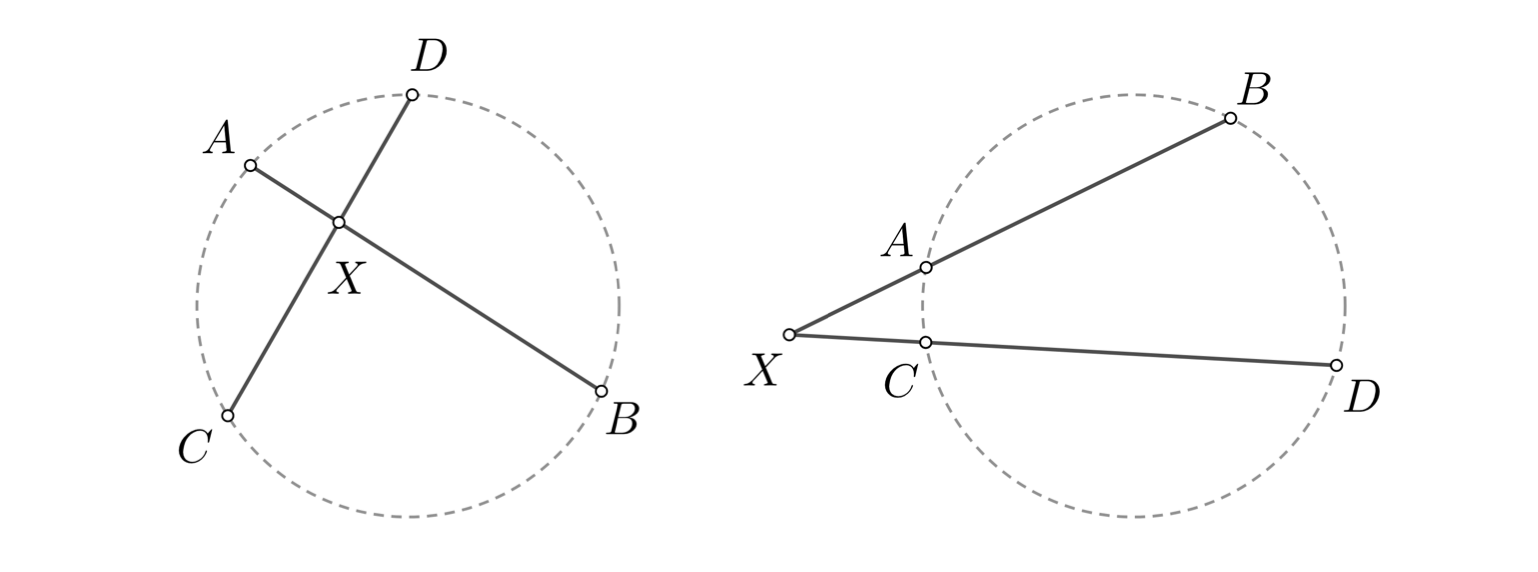
\includegraphics[width=0.8\textwidth]{ЭлМШ 2024-2025/IV блок/Тапиры/HW_Antiparallel+Power point.png}
\end{center}

\textbf{Утверждение.} Для обеих картинок сверху точки $A, B, C, D$ лежат на одной окружности тогда и только тогда, когда $X A \cdot X B=X C \cdot X D$.

Аналогичные утверждения верны, если секущую заменить на касательную.

\problem{1!}
Окружность, проходящая через вершины $A$ и $B$ параллелограмма $A B C D$ пересекает его диагонали в точках $P$ и $Q$. Докажите, что точки $P, Q, C$ и $D$ лежат на одной окружности.

\problem{2!}
Выпуклый четырёхугольник $A B C D$ вписан в окружность. Докажите, что прямая, соединяющая середины дуг $A B$ и $C D$, не содержащих отмеченных точек, перпендикулярна одной из биссектрис угла между прямыми $A B$ и $C D$.

\problem{3!}
Диагонали вписанного четырехугольника $A B C D$ пересекаются в точке К. Докажите, что касательная в точке К к окружности, описанной около треугольника $A B K$, параллельна $C D$.

\newpage

\hspace{3mm}

\centerline{\bf \Huge Power point}
\centerline{\bf \Huge }

\begin{flushright}
        \scriptsize{Ставлю хату, что Герман не решит ни одну из 4-6.}
\end{flushright}

\problem{4}\textbf{Очень важная задача!}
К окружностям $\omega_1$ и $\omega_2$ провели две общие внешние касательные $AB$ и $CD$ ($A$ и $C$ касаются окружности $\omega_1$, а $B$ и $D$ окружности $\omega_2$). Пусть прямая $AD$ пересекает окружность $\omega_1$ в точке $X$ и окружность $\omega_2$ в точке $Y$. Докажите, что $AX = DY$. Сформулируйте и докажите аналогичный факт для внутренних касательных.

\problem{5}
Точка $I$ - центр вписанной окружности треугольника $A B C$, точка $D$ - основание биссектрисы из вершины $A$. Прямая, проходящая через точку $D$ пересекает окружность, описанную около треугольника $B I C$ в точках $X$ и $Y$. Докажите, что $\angle X A B=\angle Y A C$.

\problem{6}
Четырёхугольник $A B C D$ вписан в окружность $\gamma$. Оказалось, что окружности, построенные на отрезках $A B$ и $C D$ как на диаметрах, касаются друг друга внешним образом в точке $S$. Пусть точки $M$ и $N$ - середины отрезков $A B$ и $C D$ соответственно. Докажите, что перпендикуляр $\ell$ к прямой $M N$, восставленный в точке $M$, пересекает прямую $C S$ в точке, лежащей на $\gamma$.